% Robustness Report, Journal of Robustness Reports (SciPost JRR template).
% Build: tectonic robustness_report.tex  (or pdflatex + bibtex, twice)
% The figure is produced by R/08_report_figure.R, which writes
% output/figures/08_report_figure.pdf and copies it to report/fig_main.pdf for
% the include below. Never edited by hand.
%
% Sign convention throughout: positive favours face-to-face CBT.
% Word budget: 500 words for Goal to Conclusion (Abstract, title page,
% Acknowledgments and Disclosures, References and captions are excluded).
% JRR allows ONE display element: Figure 1 (R/08_report_figure.R), which
% stacks the corrected input table (panel A) on the specification curve
% (panel B). The standalone tables (report/table_corrected.tex,
% report/table_sources.tex) go to the online supplement.

\documentclass{JRR}
\usepackage{doi}
% numbers.tex: generated by R/05_report_numbers.R from output/tables/. Do not edit.
% generated 2026-10-05 14:16
\newcommand{\krPub}{-0.20}
\newcommand{\krPubLb}{-0.44}
\newcommand{\krPubUb}{0.05}
\newcommand{\krRep}{-0.20}
\newcommand{\krRepLb}{-0.44}
\newcommand{\krRepUb}{0.05}
\newcommand{\krRepQ}{41.88}
\newcommand{\krRepItwo}{69}
\newcommand{\krHkLb}{-0.13}
\newcommand{\krHkUb}{0.53}
\newcommand{\krOurAxis}{0.20}
\newcommand{\krOurAxisLb}{-0.05}
\newcommand{\krOurAxisUb}{0.44}
\newcommand{\krInMv}{0.20}
\newcommand{\krInMvLb}{-0.05}
\newcommand{\krInMvUb}{0.45}
\newcommand{\nSrcRows}{28}
\newcommand{\nKrAgreePost}{20}
\newcommand{\nKrAgreeN}{12}
\newcommand{\nOursAgreeKrPre}{26}
\newcommand{\nOursAgreeKrPost}{22}
\newcommand{\tOneDlItwo}{68}
\newcommand{\nCiExclFtf}{12}
\newcommand{\mvRange}{0.40}
\newcommand{\mvIqr}{0.08}
\newcommand{\mdCorr}{0.20}
\newcommand{\mdOurs}{0.17}
\newcommand{\mdKris}{0.19}
\newcommand{\dsMaxShift}{0.03}
\newcommand{\mvMaxAbs}{0.36}
\newcommand{\nWithinHalfCorr}{0}
\newcommand{\mineKr}{0.20}
\newcommand{\mineKrLb}{-0.04}
\newcommand{\mineKrUb}{0.45}
\newcommand{\minePost}{0.15}
\newcommand{\minePostLb}{-0.09}
\newcommand{\minePostUb}{0.39}
\newcommand{\nArms}{28}
\newcommand{\nArmsMatch}{27}
\newcommand{\nSpecs}{2388}
\newcommand{\nCiZero}{2376}
\newcommand{\nFavourEcbt}{0}
\newcommand{\mvMin}{-0.04}
\newcommand{\mvMax}{0.36}
\newcommand{\mvMedian}{0.17}
\newcommand{\mvQa}{0.13}
\newcommand{\mvQb}{0.21}
\newcommand{\noMgMedian}{0.05}
\newcommand{\noMgMin}{-0.04}
\newcommand{\noMgMax}{0.15}
\newcommand{\otherFactorMaxShift}{0.12}
\newcommand{\tOneEst}{0.11}
\newcommand{\tOneLb}{-0.17}
\newcommand{\tOneUb}{0.38}
\newcommand{\tOneDlEst}{0.10}
\newcommand{\tOneDlLb}{-0.13}
\newcommand{\tOneDlUb}{0.33}
\newcommand{\noMgItwo}{0}
\newcommand{\pctCiZero}{99.5}
\newcommand{\primaryEst}{0.16}
\newcommand{\primaryLb}{-0.12}
\newcommand{\primaryUb}{0.45}
\newcommand{\primaryHkLb}{-0.21}
\newcommand{\primaryHkUb}{0.53}
\newcommand{\repOrig}{-1.73}
\newcommand{\repOrigLb}{-2.72}
\newcommand{\repOrigUb}{-0.74}
\newcommand{\repOrigItwo}{98}
\newcommand{\repCorr}{-0.92}
\newcommand{\repCorrLb}{-1.76}
\newcommand{\repCorrUb}{-0.09}
\newcommand{\repCorrItwo}{97}
\newcommand{\repAddm}{-0.79}
\newcommand{\repAddmLb}{-1.61}
\newcommand{\repAddmUb}{0.02}
\newcommand{\pubOrig}{-1.73}
\newcommand{\pubOrigLb}{-2.72}
\newcommand{\pubOrigUb}{-0.74}
\newcommand{\pubAddm}{-0.79}
\newcommand{\pubAddmLb}{-1.60}
\newcommand{\pubAddmUb}{0.02}
\newcommand{\pubCorr}{-0.92}
\newcommand{\pubCorrLb}{-1.76}
\newcommand{\pubCorrUb}{-0.09}
  % generated by R/05_report_numbers.R

\graphicspath{{../output/figures/}}

\begin{document}
%TC:ignore
\pagestyle{SPstyle}

\noindent
{\bfseries \LARGE
Standard errors entered as standard deviations: four analyses of electronic versus face-to-face cognitive behavioural therapy in Luo et al.\ (2020), its addendum, corrigendum and letter of concern
\par}

\vspace{1em}

\noindent
\begin{minipage}[t]{0.7\textwidth}
\vspace{0pt}
{\it
Constantin Yves Plessen\textsuperscript{1$\star$}
}\\[0.5em]
{\bf 1} Psychotherapy and Psychotherapy Research (CBT), Center for Psychotherapy, University of Graz, Graz, Austria
\\[0.5em]
$\star$ \href{mailto:constantin.plessen@uni-graz.at}{\small constantin.plessen@uni-graz.at}
\\[1em]
\end{minipage}
\hspace{1em}
\begin{minipage}[t]{0.3\textwidth}
    \vspace{-10pt}
    \raggedleft
    
\includegraphics[width=1\textwidth]{LOGO_JRR_1_COLOR.png}
\end{minipage}

\section*{Abstract}
\textbf{\boldmath{%
All four published estimates recompute from their inputs; only the letter's inputs are standard deviations. \nSpecs{} specifications give $g$ from $\mvMin$ to $\mvMax$; no interval favours eCBT.
}}

\vspace{\baselineskip}

\noindent\textcolor{white!90!black}{%
\fbox{\parbox{0.975\linewidth}{%
\textcolor{white!40!black}{\begin{tabular}{lr}%
  \begin{minipage}{0.6\textwidth}%
    {\small Copyright attribution to authors. \newline
    This work is a submission to Journal of Robustness Reports. \newline
    License information to appear upon publication. \newline
    Publication information to appear upon publication.}
  \end{minipage} & \begin{minipage}{0.4\textwidth}
    {\small Received Date \newline Accepted Date \newline Published Date}%
  \end{minipage}
\end{tabular}}
}}
}

\linenumbers

\section*{Target article}
\bibentry{luo2020}
%TC:endignore

\section{Goal}
\label{sec:goal}

The target pooled 14 trials of electronic (eCBT) against face-to-face cognitive behavioural therapy for depression: $\pubOrig$ [95\% CI $\pubOrigLb$, $\pubOrigUb$], $I^2 = 98\%$, read as eCBT more effective \cite{luo2020}. An addendum reinterpreted it as less change for eCBT \cite{luo2020addendum}; a corrigendum gave $\pubCorr$ [$\pubCorrLb$, $\pubCorrUb$] and declared its conclusions unchanged \cite{sanger2021corrigendum}, although the original abstract still claims the opposite; a letter of concern re-extracted the trials and found $\krOurAxis$ [$\krOurAxisLb$, $\krOurAxisUb$] \cite{kriston2022concerns} (positive favours face-to-face CBT throughout; the letter prints the opposite sign). I asked whether each estimate follows from its document's inputs, and how robust the effect is.

\section{Methods}
\label{sec:methods}

I recomputed each estimate from its document's inputs; reproduction means agreement at printed precision. I re-extracted all trials from the primary reports and cross-checked against both published extractions. Hedges' $g$ was pooled with metafor \cite{viechtbauer2010metafor} in a metaMultiverse \cite{plessen2026metamultiverse} specification curve \cite{simonsohn2020specification, plessen2023multiverse} over six factors: data source (corrigendum, letter, mine), effect-size metric \cite{becker1988, morris2008}, instrument, inclusion set, estimator and the handling of the change-score-only trial \cite{wright2005}.

\section{Results}
\label{sec:results}

Kriston et al.\ identified each arm's entered ``SD'' as the standard error (SE) of the mean change \cite{kriston2022concerns}. I confirm it in \nArmsMatch{} of \nArms{} arms; RevMan's formula on these entries returns $\pubOrig$, $\pubAddm$ and $\pubCorr$ exactly, with $I^2$ of \repCorrItwo{} to $\repOrigItwo\%$. The letter's estimate reproduces exactly from its supplement.

Two findings are not in the letter of concern. First, Wright 2005 \cite{wright2005} reports baseline and change scores only. The original correctly derived the post-treatment mean as baseline minus endpoint change; the corrigendum ``corrected'' it to the week-4 completer change score, wrong column and time point, which the letter did not report. Second, the inconsistency for which the original downgraded its evidence is an artefact of the SEs: with SDs, $I^2$ is $\tOneDlItwo\%$ (Figure~\ref{fig:main}A), $\noMgItwo\%$ without the MoodGYM trials. Across \nSpecs{} specifications (Figure~\ref{fig:main}B) over three data sources, $g$ spans $\mvMin$ to $\mvMax$ (median $\mvMedian$, IQR $\mvQa$ to $\mvQb$); only \nCiExclFtf{} intervals exclude zero, all favouring face-to-face CBT. Data source shifts the median by at most $\dsMaxShift$: with SDs, the corrigendum's table gives $\tOneDlEst$ [$\tOneDlLb$, $\tOneDlUb$], my re-extraction $\minePost$ [$\minePostLb$, $\minePostUb$], or $\mineKr$ [$\mineKrLb$, $\mineKrUb$] under the letter's specification. Inclusion is the largest source of spread: without the MoodGYM trials ($n = 19$, $44$) the median is $\noMgMedian$; no other factor shifts it by more than $\otherFactorMaxShift$. No specification comes within $0.5$ of the published $\pubCorr$.

\begin{figure}[p]
\centering
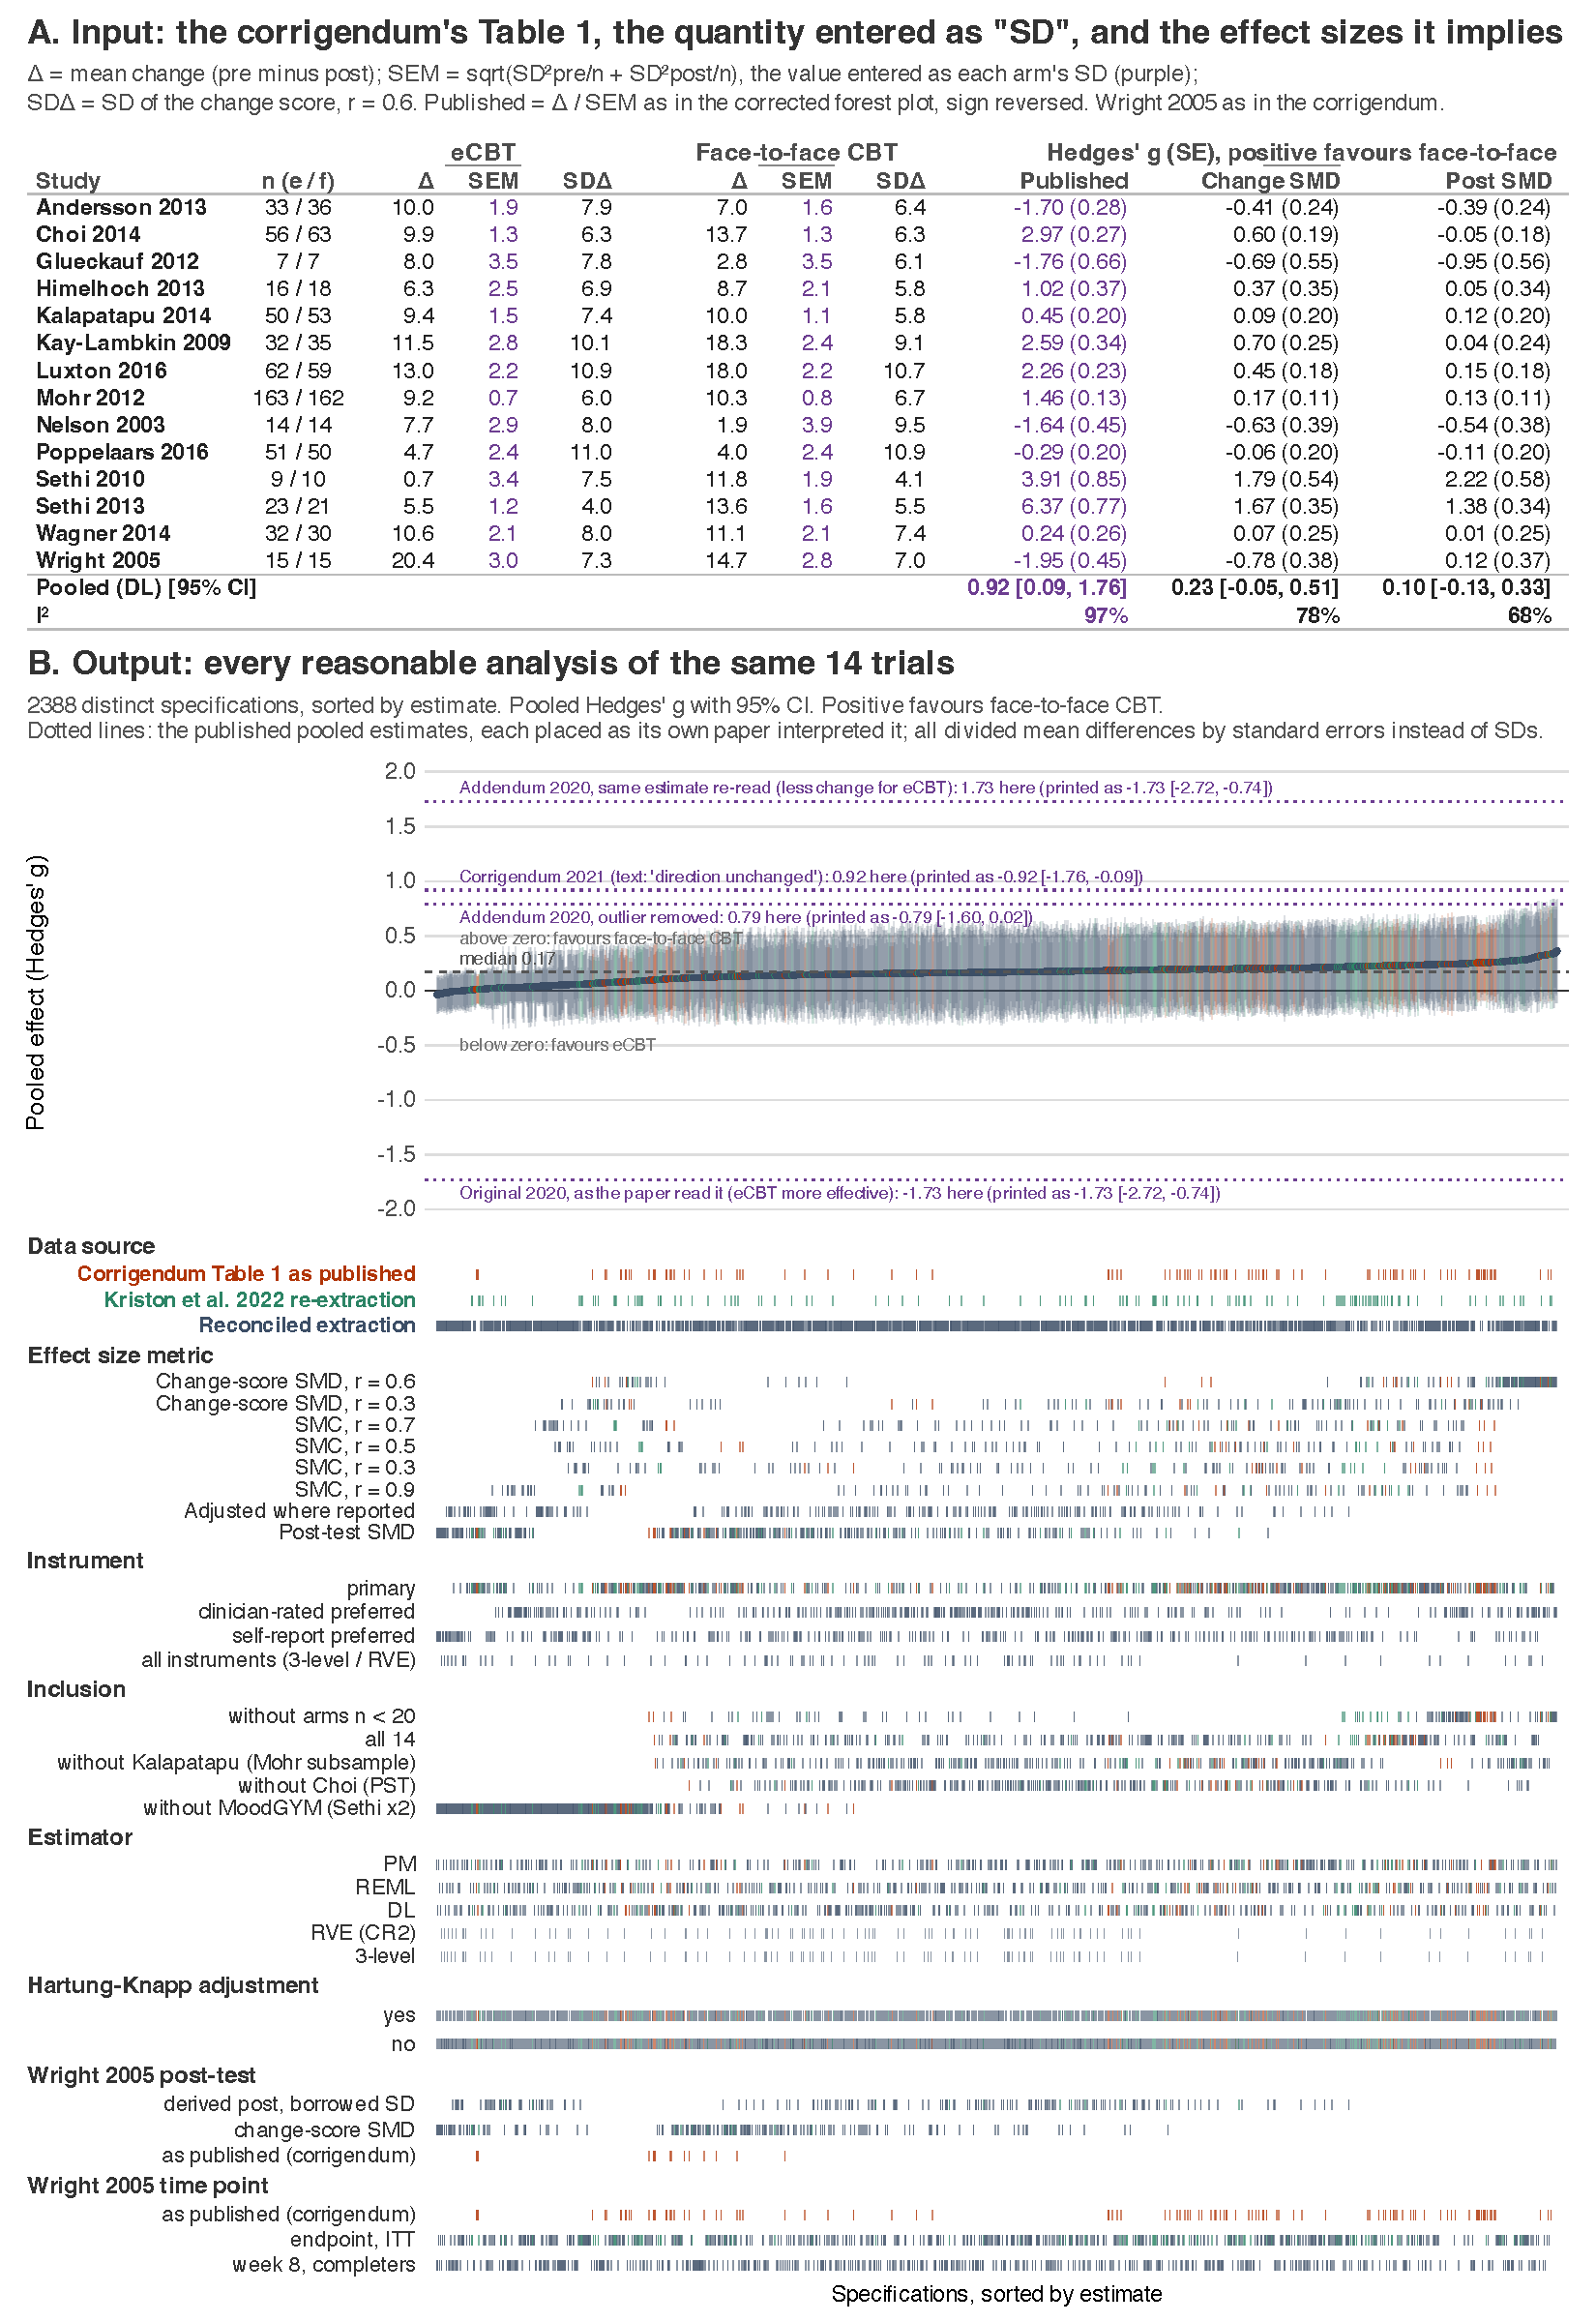
\includegraphics[width=0.78\linewidth]{fig_main}
\caption{\label{fig:main} Input and output of the reanalysis. \textbf{A}: the corrigendum's Table 1 per study. $\Delta$ is the mean change (pre minus post); SEM $= \sqrt{\mathrm{SD}_\mathrm{pre}^2/n + \mathrm{SD}_\mathrm{post}^2/n}$ is what the authors entered as each arm's ``SD'' (purple); SD$_\Delta$ is the SD of the change score at pre-post $r = 0.6$, the value Luxton 2016 reports. Effect sizes are Hedges' $g$ (SE), positive favouring face-to-face CBT: published ($\Delta$/SEM, sign reversed from the printed plot), change-score SMD, post-test SMD; pooled rows are DerSimonian-Laird. \textbf{B}: pooled $g$ with 95\% CI for \nSpecs{} distinct specifications sorted by estimate, coloured by data source (named in the same colours in the first dashboard block), with the published estimates placed as each paper read them (dotted) and each specification's factor levels below. Change-score SMD uses $r \in \{0.3, 0.6\}$ (the letter's value; Luxton's), standardised mean change $r \in \{0.3, 0.5, 0.7, 0.9\}$. Levels implied by other rows are omitted. Full table and source comparison: online supplement.}
\end{figure}

\section{Conclusion}
\label{sec:conclusion}

All four published estimates recompute exactly from their printed inputs, but the original, addendum and corrigendum are obtained only by entering standard errors as standard deviations; with SDs, three independent extractions and every defensible analysis give estimates not comparable in magnitude to the published ones. This reanalysis undercuts the target's claim that eCBT is more effective and the corrigendum's claim of unchanged conclusions; it corroborates the letter. As in the letter, every quantity changes once SDs replace SEs: estimates, intervals, heterogeneity. The interval includes zero in $\pctCiZero\%$ of specifications: the evidence is compatible with small differences in either direction; the slight advantage for face-to-face CBT rests on two small MoodGYM trials.

%TC:ignore
\section*{\large{Acknowledgments and Disclosures}}
\label{sec:code}

\paragraph{Reproducibility}
For each of the four documents: \emph{Original} \cite{luo2020}: the printed $\pubOrig$ [$\pubOrigLb$, $\pubOrigUb$] is recovered exactly from the forest-plot inputs with DerSimonian-Laird and RevMan's variance, but those inputs are standard errors, so the recovered value is not a standardised mean difference. \emph{Addendum} \cite{luo2020addendum}: its re-reading of $\pubOrig$ is the same number, and its $\pubAddm$ [$\pubAddmLb$, $\pubAddmUb$] with Choi 2014 removed recovers to within rounding, with the same caveat; its post-intervention analysis ($0.21$ [$-0.05$, $0.46$]) could not be reproduced: the corrigendum's table gives $0.10$ [$-0.13$, $0.33$] (DerSimonian-Laird, RevMan variance) and the pre-correction values in the corrigendum's footnotes give $0.14$ [$-0.13$, $0.40$], or $0.19$ [$-0.09$, $0.46$] without Choi 2014. \emph{Corrigendum} \cite{sanger2021corrigendum}: $\pubCorr$ [$\pubCorrLb$, $\pubCorrUb$] recovers exactly from its forest-plot values, which disagree with its own Table 1 in four cells and whose Wright 2005 entries are week-4 change scores; the computation is correct but the inputs are standard errors. \emph{Letter of concern} \cite{kriston2022concerns}: the printed $\krPub$ [$\krPubLb$, $\krPubUb$], $Q = \krRepQ$, $I^2 = \krRepItwo\%$, reproduces exactly from its supplementary table with DerSimonian-Laird, change-score SMD at $r = 0.3$ and RevMan's small-sample correction; all 14 per-study values match at two decimals, and the pooled estimate is stable under REML (Hartung-Knapp interval $\krHkLb$ to $\krHkUb$, positive favouring face-to-face). No authors' reply to the letter was found.

\paragraph{Code and Data Availability}
All data (published tables, screenshots of the primary-study tables, the reconciled extraction with per-value provenance), numbered R scripts, outputs and an extended version of this report are in the FAIR \cite{wilkinson2016fair} repository at \url{https://doi.org/10.5281/zenodo.XXXXXXX} (GitHub: \url{https://github.com/cyplessen/ecbt-fcbt-reanalysis}). Effect sizes were computed with metafor \cite{viechtbauer2010metafor}; the specification curve used metaMultiverse \cite{plessen2026metamultiverse}, whose pre-post effect-size support (version 0.3.1) was developed for this reanalysis; the project-level implementation is included in the repository. The letter's supplementary workbook is transcribed verbatim in \texttt{data/}.

\paragraph{Author Contributions}
\textbf{C.Y.P.:} Conceptualization, Data curation, Formal analysis, Investigation, Methodology, Software, Visualization, Writing - original draft, Writing - review \& editing.

\paragraph{Funding}
The author received no financial support for the research, authorship, and/or publication of this article.

\paragraph{Conflicts of Interest}
The author maintains the metaMultiverse R package used in the analysis \cite{plessen2026metamultiverse}, and published two blog posts on the target article in 2020, since removed, which served as extraction records for this work. No other competing interests.

\bibliography{references}

%TC:endignore
\end{document}
